\subsection{Darlington Schaltung} % (fold)
\label{sub:Darlington_Schaltung}
\begin{frame}
    \frametitle{Darlington Schaltung}
    \framesubtitle{Schaltung}
    \begin{figure}[H]
    \begin{center}
            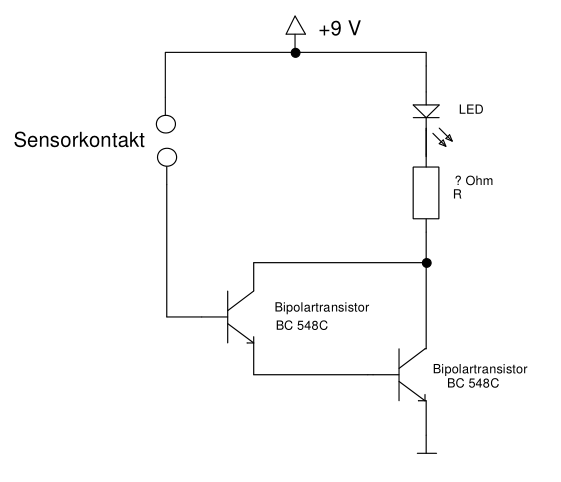
\includegraphics[scale=0.4]{./img/schaltungen/darlington.png}
    \end{center}
    \end{figure}
\end{frame}
\begin{frame}
    \frametitle{Darlington Schaltung}
    \framesubtitle{}
    \begin{columns}[c]
    \column{0.5\textwidth}
        \begin{figure}[H]
        \begin{center}
                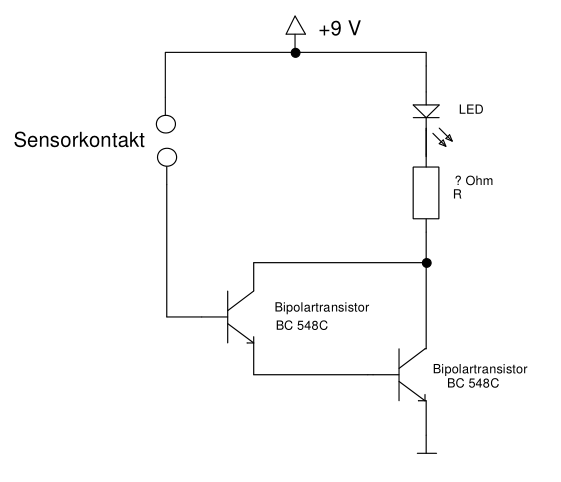
\includegraphics[scale=0.3]{./img/schaltungen/darlington.png}
        \end{center}
        \end{figure}
    \column{0.5\textwidth}
    \begin{block}{Widerstände}
     \begin{itemize}
         \item Widerstand wie bei LED-Schaltung $R = 470 \Omega$
         \item Widerstand durch Finger: Hoher Körperwiderstand um starke
         Basisströme zu vermeiden
     \end{itemize}
    \end{block}
    \end{columns}
\end{frame}
\begin{frame}
    \frametitle{Darlington Schaltung}
    \framesubtitle{}
    \begin{columns}[c]
    \column{0.5\textwidth}
        \begin{figure}[H]
        \begin{center}
                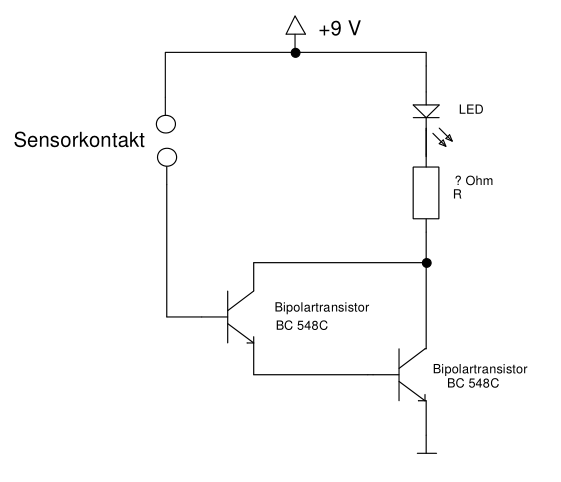
\includegraphics[scale=0.3]{./img/schaltungen/darlington.png}
        \end{center}
        \end{figure}
    \column{0.5\textwidth}
    \begin{block}{Funktionsweise}
     \begin{itemize}
        \item Verstärkung von kleinen Strömen durch Iteration von Transistoren
        \item Gesamtverstärkung $B \approx B_1 \cdot B_2$
     \end{itemize}
    \end{block}
    \end{columns}
\end{frame}
% section Darlington Schaltung (end)
